\documentclass{standalone}
\usepackage{graphicx}	
\usepackage{amssymb, amsmath, amsthm}
\usepackage{color}

\usepackage{tikz}
\usetikzlibrary{math}

\definecolor{light}{RGB}{220, 188, 188}
\definecolor{mid}{RGB}{185, 124, 124}
\definecolor{dark}{RGB}{143, 39, 39}
\definecolor{highlight}{RGB}{180, 31, 180}
\definecolor{lightteal}{RGB}{107, 142, 142}
\definecolor{midteal}{RGB}{72, 117, 117}
\definecolor{darkteal}{RGB}{29, 79, 79}
\definecolor{gray10}{gray}{0.1}
\definecolor{gray20}{gray}{0.2}
\definecolor{gray30}{gray}{0.3}
\definecolor{gray40}{gray}{0.4}
\definecolor{gray60}{gray}{0.6}
\definecolor{gray70}{gray}{0.7}
\definecolor{gray80}{gray}{0.8}
\definecolor{gray90}{gray}{0.9}
\definecolor{gray95}{gray}{0.95}

\begin{document}

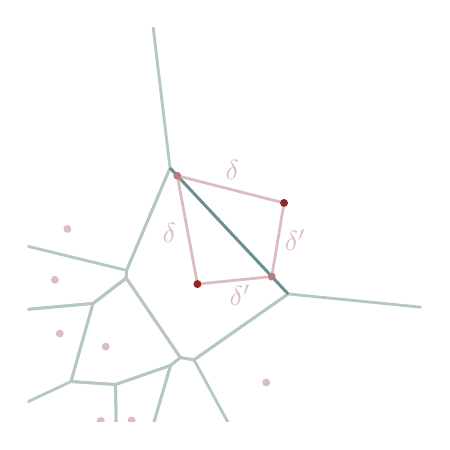
\begin{tikzpicture}[scale=2]
  \clip (-0.75, -0.75) rectangle (1.75, 1.75);
  
  \fill[white] (-2, -2) rectangle (2, 2);
   
  \colorlet{custom}{lightteal!50!white};
  
  \draw[custom, line width=1] (-0.475, -0.497)
    \foreach \x/\y in {-0.475/-0.497, -0.192/-0.516, 
                       0.157/-0.395, 0.220/-0.345, -0.124/0.160, 
                      -0.335/-0.001, -0.475/-0.497} {
      -- (\x, \y)
  };
  
  \draw[custom, line width=1] (-0.251, -2.000)
    \foreach \x/\y in {-0.251/-2.000, -0.176/-1.538, -0.192/-0.516, -0.475/-0.497} {
      -- (\x, \y)
  };
  
  \draw[custom, line width=1] (1.197, -2.000)
    \foreach \x/\y in {1.197/-2.000, 0.306/-0.359, 0.220/-0.345, 0.157/-0.395, -0.176/-1.538} {
      -- (\x, \y)
  };
  
  \draw[custom, line width=1] (2.000, -0.050)
    \foreach \x/\y in {2.000/-0.050, 0.904/0.059, 0.306/-0.359} {
      -- (\x, \y)
  };
  
  \draw[custom, line width=1] (0.017, 2.000)
    \foreach \x/\y in {0.017/2.000, 0.154/0.859, 0.904/0.059} {
      -- (\x, \y)
  };
  
  \draw[custom, line width=1] (-2.000, 0.666)
    \foreach \x/\y in {-2.000/0.666, -0.122/0.209, 0.154/0.859} {
      -- (\x, \y)
  };
  
  \draw[custom, line width=1] (-2.000, -0.151)
    \foreach \x/\y in {-2.000/-0.151, -0.335/-0.001, -0.124/0.160, -0.122/0.209} {
      -- (\x, \y)
  };
  
  \draw[custom, line width=1] (-2.000, -0.151)
    \foreach \x/\y in {-2.000/-0.151, -0.335/-0.001, -0.124/0.160, -0.122/0.209} {
      -- (\x, \y)
  };
  
  \draw[custom, line width=1] (-2.000, -1.212)
    \foreach \x/\y in {-2.000/-1.212, -0.475/-0.497, -0.335/-0.001} {
      -- (\x, \y)
  };
  
  \draw[custom, line width=1] (-0.122, 0.209)
    \foreach \x/\y in {-0.122/0.209, -0.124/0.160, 0.220/-0.345, 
                        0.306/-0.359, 0.904/0.059, 0.154/0.859, -0.122/0.209} {
      -- (\x, \y)
  };
  
  \draw[custom, line width=1] (-0.176, -1.538)
    \foreach \x/\y in {-0.176/-1.538, 0.157/-0.395, -0.192/-0.516, -0.176/-1.538} {
      -- (\x, \y)
  };
  
  \foreach \x/\y in {-0.498/0.472, -0.546/-0.192, -0.286/-0.747, 
                     0.765/-0.503, 0.878/0.637, -0.577/0.149, 
                     -0.254/-0.275, 0.328/0.122, 0.177/-0.822, -0.090/-0.744} {
    \fill[light] (\x, \y) circle (0.025);
  }
  
  \draw[lightteal, line width=1] (0.904, 0.059) -- (0.154, 0.859);

  \pgfmathsetmacro{\xa}{0.878}
  \pgfmathsetmacro{\ya}{0.637}

  \pgfmathsetmacro{\xb}{0.328}
  \pgfmathsetmacro{\yb}{0.122}
  
  \pgfmathsetmacro{\xab}{(\xa + \xb) / 2}
  \pgfmathsetmacro{\yab}{(\ya + \yb) / 2}
  
  \pgfmathsetmacro{\mab}{ ( \yb - \ya ) / ( \xb - \xa ) }
  \pgfmathsetmacro{\mabp}{-1 / \mab}
  
  \pgfmathsetmacro{\xc}{0.2}
  \pgfmathsetmacro{\yc}{\mabp * (\xc - \xab ) + \yab }
  \pgfmathsetmacro{\r}{ sqrt( (\xc - \xa) * (\xc - \xa) + (\yc - \ya) * (\yc - \ya) ) }
  
  \draw[light, line width=1] (\xa, \ya) -- (\xc, \yc) -- (\xb, \yb);
  \fill[mid] (\xc, \yc) circle (0.025);
  
  \node[light] at (0.15, 0.45) { $\delta$ };
  \node[light] at (0.55, 0.85) { $\delta$ };
    
  \pgfmathsetmacro{\xc}{0.8}
  \pgfmathsetmacro{\yc}{\mabp * (\xc - \xab ) + \yab }
  \pgfmathsetmacro{\r}{ sqrt( (\xc - \xa) * (\xc - \xa) + (\yc - \ya) * (\yc - \ya) ) }
  
  \draw[light, line width=1] (\xa, \ya) -- (\xc, \yc) -- (\xb, \yb);
  \fill[mid] (\xc, \yc) circle (0.025);
  
  \node[light] at (0.6, 0.05) { $\delta'$ };
  \node[light] at (0.95, 0.4) { $\delta'$ };
  
  \foreach \x/\y in { 0.878/0.637, 0.328/0.122 } {
    \fill[dark] (\x, \y) circle (0.025);
  }
  
\end{tikzpicture}

\end{document}  